\chapter{Data format for Benchmark Results}
\label{chap:data-format}
\futureinversion{1.0}{The information in this section will be updated according to the implementation.}
This appendix shows an example of Graphalytics benchmark results of the reference implementation. Graphalytics benchmark defines a specific data format for the benchmark results. The result is formatted in JSON, and consists of three main components: system under test, benchmark configuration, and experimental results. Figure~\ref{fig:result-format:overview} depicts the top-level structure of the result format.

\begin{figure}[h]
	\centering
	\caption{Result Format: Overview}
	\fbox{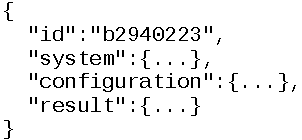
\includegraphics[width=0.3\linewidth]{figures/data-format.pdf}}
	\label{fig:result-format:overview}
\end{figure}

For the system under test, Graphalytics reports the detailed descriptions of the graph analytic platform, the cluster environment, and the benchmark tool.

\begin{figure}[!h]
	\centering
	\caption{Result Format: System Under Test}
	\fbox{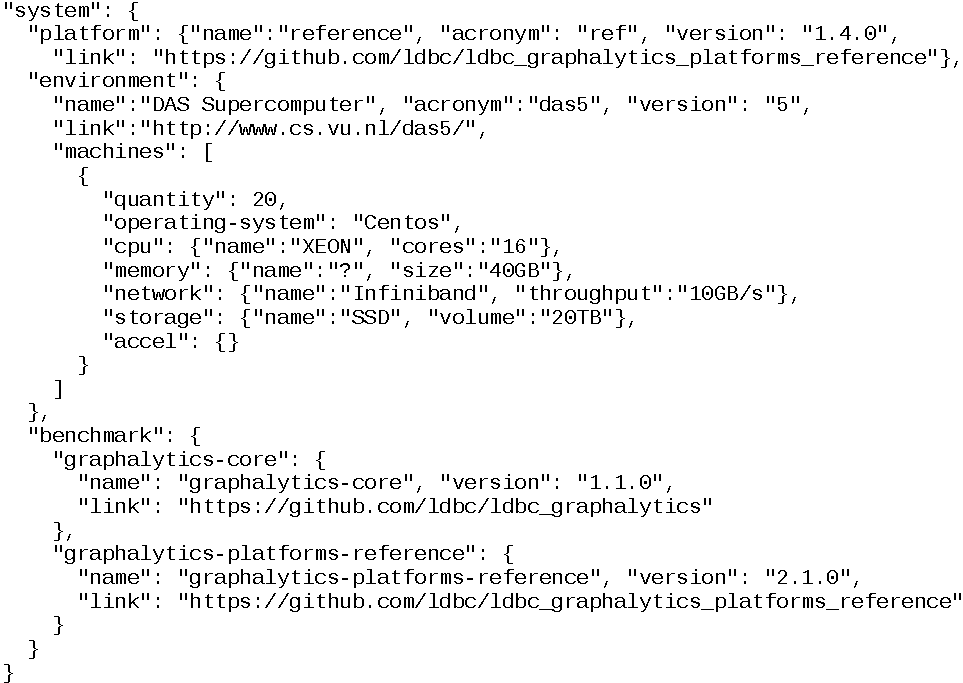
\includegraphics[width=1.0\linewidth]{figures/data-format-system.pdf}}
	\label{fig:result-format:system}
\end{figure}

For the benchmark configuration, the target scale and the computation resource usage is reported. For each resource type, the baseline resource usage, and the scalablity of that resource type is reported.

\begin{figure}[!h]
	\centering
	\caption{Result Format: Benchmark Configuration}
	\fbox{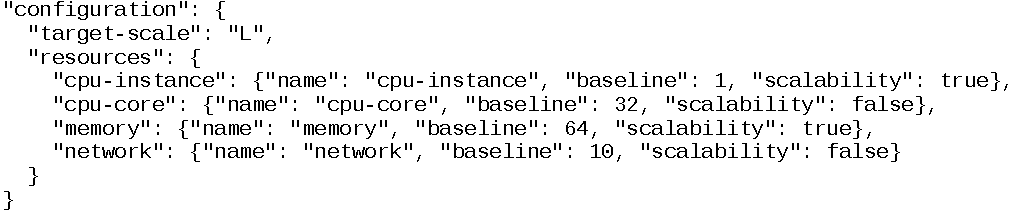
\includegraphics[width=1.0\linewidth]{figures/data-format-conf.pdf}}
	\label{fig:result-format:conf}
\end{figure}

\begin{figure}[!h]
	\centering
	\caption{Result Format: Experiment Result}
	\fbox{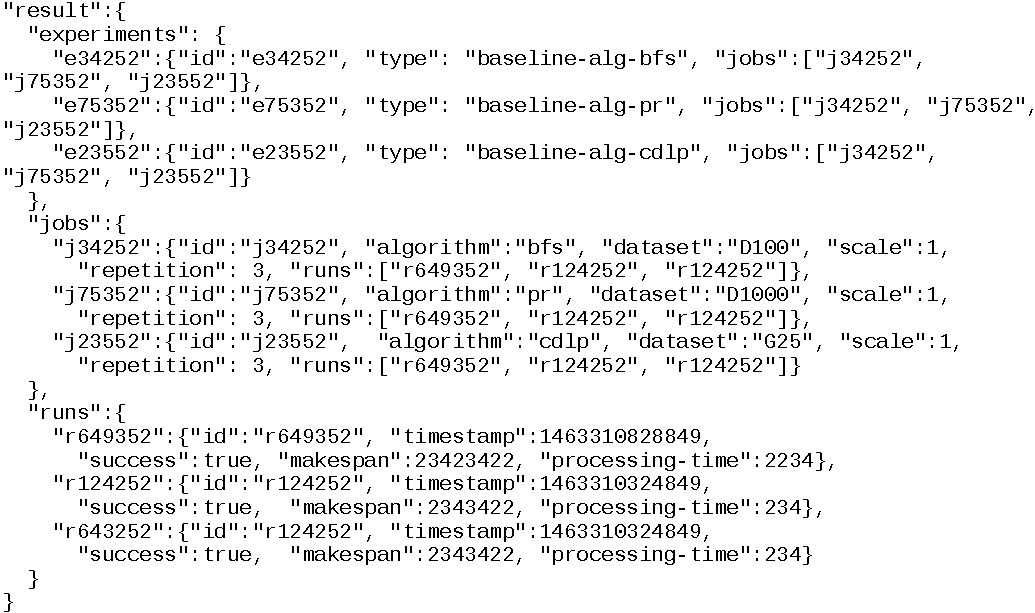
\includegraphics[width=1.0\linewidth]{figures/data-format-result.pdf}}
	\label{fig:result-format:result}
\end{figure}

For the experimental results, the set of experiments, the underlying jobs, and the corresponding runs are reported.
